% !TEX TS-program = pdflatex
% !TEX encoding = UTF-8 Unicode



\documentclass[11pt,a4paper]{article}

\usepackage[francais]{babel}
\usepackage[T1]{fontenc}
\usepackage[utf8]{inputenc}

\usepackage{amsmath,amsfonts,amssymb}

\usepackage{geometry}
\geometry{margin=75pt}

\usepackage[upright]{fourier}

\usepackage{hyperref}

\usepackage{shadethm}

\usepackage{pgf,tikz}
\usetikzlibrary{arrows}

\usepackage{color}
\definecolor{gris_clair}{gray}{.9}
\definecolor{gris}{gray}{.35}
\definecolor{vert}{rgb}{0,0.5,0}
\definecolor{rouge}{rgb}{0.5,0,0}
\definecolor{turquoise}{rgb}{0,0.5,0.5}

\usepackage{listings}           
\lstset{
language=Python,
backgroundcolor=\color{gris_clair},
frame=single,
basicstyle=\footnotesize\ttfamily\color{gris},
identifierstyle=\color{black},
keywordstyle=\color{vert},
stringstyle=\color{rouge}, showstringspaces=false,
commentstyle=\itshape\color{turquoise},
%numbers=left, numbersep=5pt, numberstyle=\color{gris}\tiny,stepnumber=5,
breaklines=true,
literate=
  {é}{{\'e}}1 {É}{{\'E}}1 {à}{{\`a}}1 {è}{{\`e}}1% 
  {À}{{\`A}}1 {È}{{\'E}}1 {ë}{{\"e}}1 {ï}{{\"i}}1%
  {â}{{\^a}}1 {ê}{{\^e}}1 {î}{{\^i}}1 {ô}{{\^o}}1% 
  {û}{{\^u}}1 {Â}{{\^A}}1 {Ê}{{\^E}}1 {Î}{{\^I}}1%
  {Ô}{{\^O}}1 {œ}{{\oe}}1 {Œ}{{\OE}}1 {æ}{{\ae}}1%
  {Æ}{{\AE}}1 {ç}{{\c c}}1 {Ç}{{\c C}}1 {€}{{\EUR}}1 ,
morekeywords={len,input,range}}         


\title{Projet ISN\\Sur le pocket cube}
\date{}
\author{Antonin Dudermel}

\begin{document}

\newshadetheorem{defin}{Définition}
\newshadetheorem{theo}{Théorème}

\maketitle

\begin{abstract}
	{\it Ce projet a été mené en binôme dans le cadre de mon baccalauréat d'option informatique. J'ai été assez surpris et touché en le relisant de me rendre compte de la naïveté avec laquelle je programmais il y a un peu moins de deux ans. La partie sur la résolution (travail de mon binôme) montre que je n'avais pas bien saisi à l'époque le principe du parcours IDA*, et quelques \href{https://xkcd.com/1833/}{maladresses} au niveau du code me font encore rougir. Il sera donc demandé au lecteur un peu d'indulgence}

Le principe de ce projet est de montrer à quelqu'un comment résoudre un 2*2*2 mélangé en un minimum de coups.
Il s'agit tout d'abord de passer du cube à l'ordinateur, pour cela il faut le photographier. 
Nous devons ensuite transcrire les images en un objet-cube informatique pour que l'ordinateur puisse l'étudier.
Cet objet nous permet de parcourir les différentes possibilités et de trouver la (les) plus courte(s).
Il nous faut enfin montrer cette solution grâce à un affichage 3D.
\end{abstract}

\section{Sur la capture}
	\subsection{Matériel utilisé}

    Pour pouvoir capturer facilement et grâce à python les images des faces nous avons opté pour une Raspberry
Pi (nano-ordinateur) liée à une caméra spécialisée, commandée avec python grâce au module picamera.
    L'intérêt de la Raspberry pi est tout d'abord d'avoir un ordinateur sous linux en tant que super-utilisateur,
ce qui permet notamment d'utiliser des installeurs pour les modules comme PIL (Python Imaging Library).
    Le module de la caméra ne disposant pas encore de tutoriels, cela a permis de d'apprendre directement à partir de la documentation.
\begin{figure}[h]
	\centering
	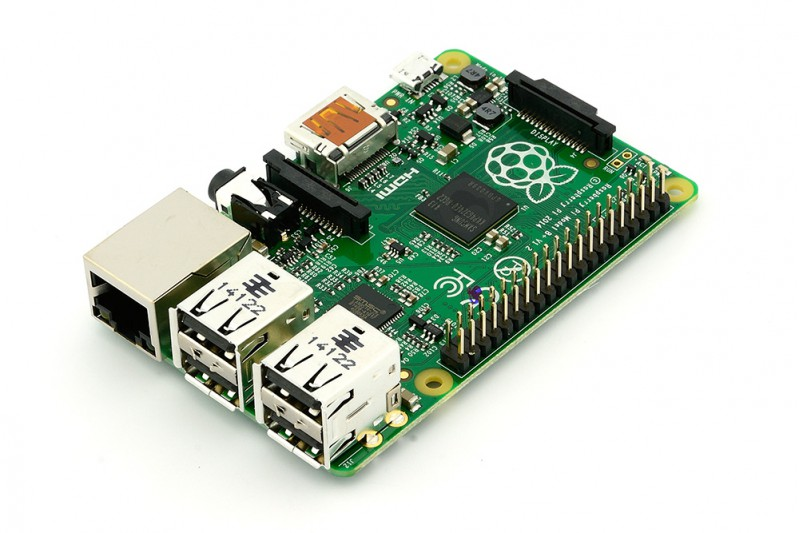
\includegraphics[scale=0.2]{Raspberry_Pi_B-_u}
	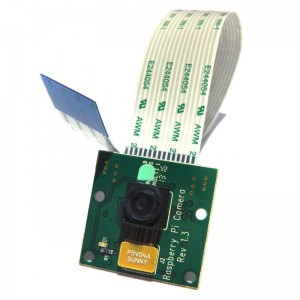
\includegraphics[scale=0.3]{raspberry-pi-camera}
	\caption{une raspberry pi B et sa caméra}
\end{figure}
La capture d'une image s'effectue avec le module \texttt{picamera}. On crée un objet \texttt{camera} dont le module \texttt{capture} permet d'enregistrer
une image PNG.
\begin{lstlisting}
import picamera
camera = picamera.PiCamera()
camera.capture("photo.jpg")
\end{lstlisting}
Pour savoir quelles parties de l'image seront utilisées, on utilise des overlays, quatre images de croix redimensionnées que l'on affiche sur l'image sortie par la caméra.
\begin{lstlisting}
img = Image.open("overlays/wikicross.png")
    pad = Image.new("RGB", (
        ((img.size[0] + 31) // 32) * 32,
        ((img.size[1] + 15) // 16) * 16,
        ))
    pad.paste(img, (0,0))
    o = [cam.add_overlay(pad.tostring(), size=img.size) for x in range(4)]
\end{lstlisting}


	\subsection{Sur la reconnaissance des couleurs}
    Une couleur peut etre représentée grace à la norme RGB. Basé sur le principe de sythèse additive des couleurs,
On donne à chaque couleur sa quantité en trois couleurs primaires : rouge,vert,bleu. Cette norme, très courante, est
utile pour représenter une image, cependant nous avons plus besoin de la teinte. Il existe une norme pour cela : la norme HLS
La norme HLS utilise aussi trois valeurs : Hue(teinte), Light(luminosité), Saturation.

\begin{figure}[h]
	\centering
	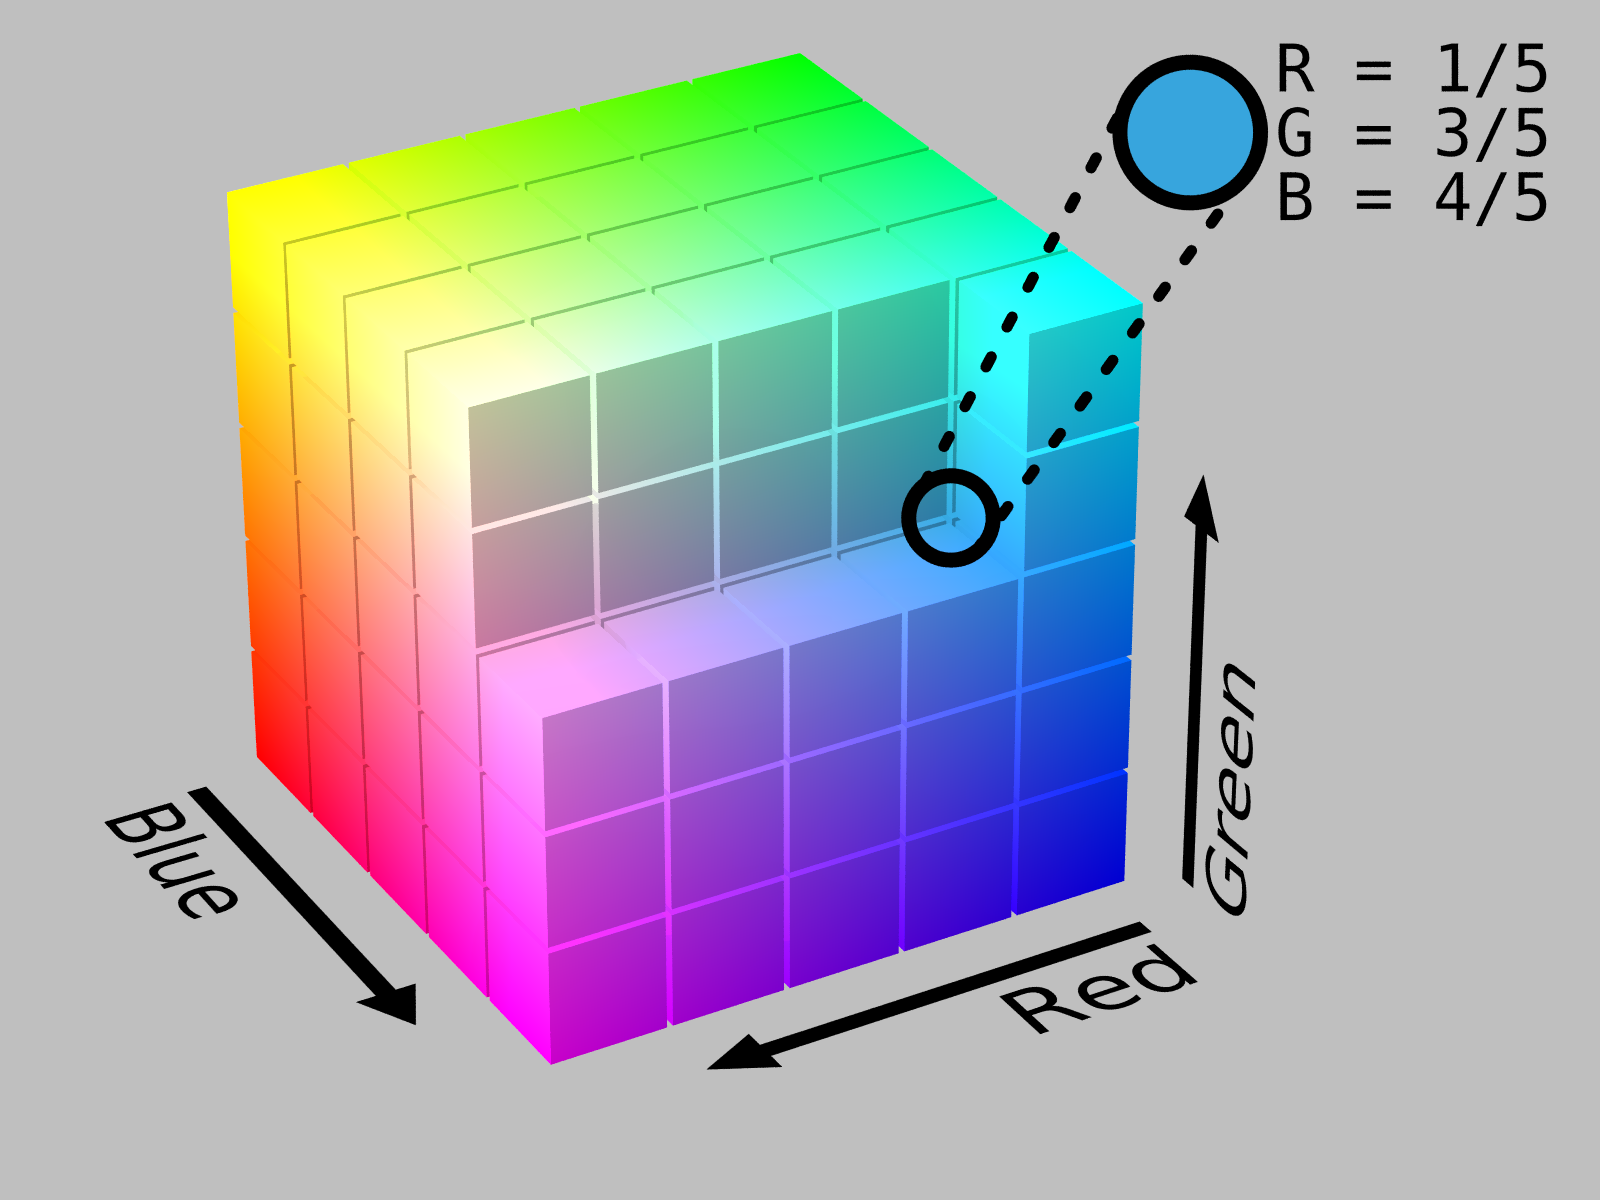
\includegraphics[scale=0.1]{RGB_Cube_Show_lowgamma_cutout_b}
	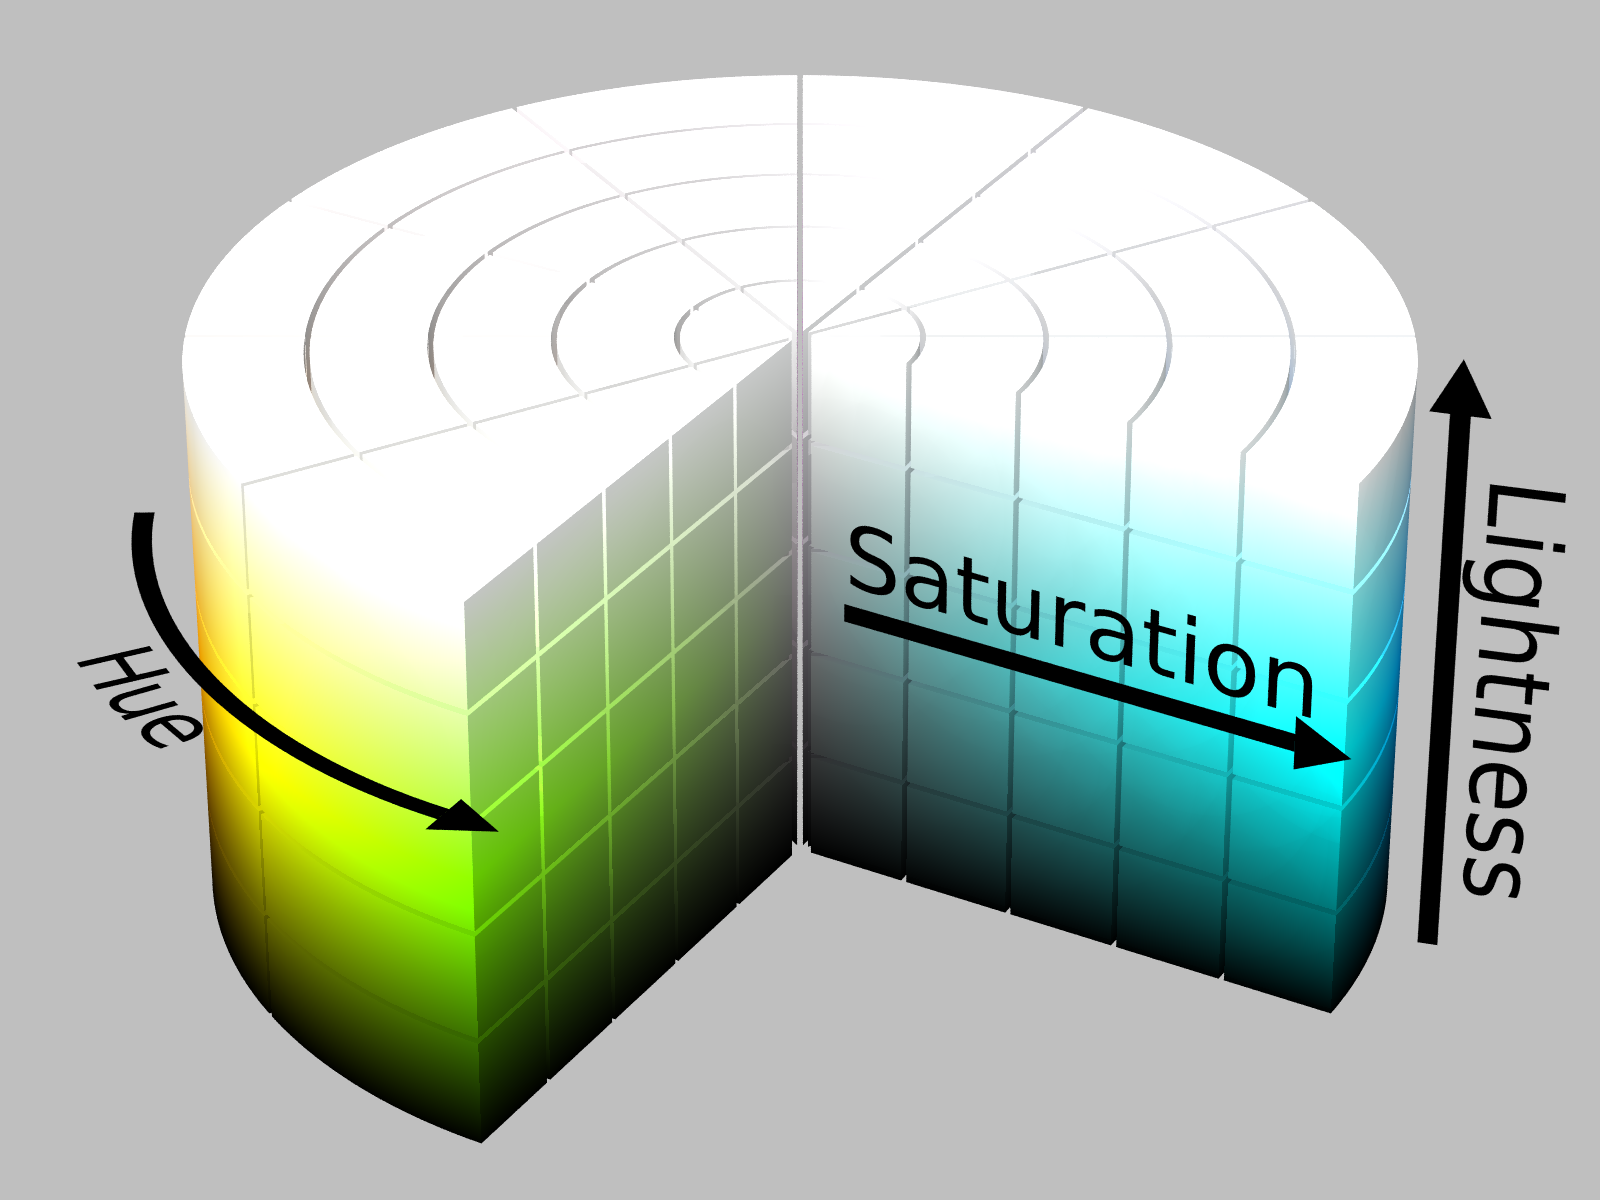
\includegraphics[scale=0.1]{HSL_color_solid_cylinder_alpha_lowgamma}
	\caption{systèmes RGB et HLS}
\end{figure}
la valeur hue est un angle : 0° ou 360° pour rouge, 120° pour vert, 240° pour bleu, cela nous permet de récupérer directement la couleur du cube
les valeurs l et s sont des valeurs numériques. Le module \texttt{colorsys} possède une fonction \texttt{rgb\_to\_hls} permettant de passer de RGB à HLS.
\begin{lstlisting}
from colorsys import rgb_to_hls
def rgb256_to_hls(pixel):
    return rgb_to_hls(*[couleur / 256 for couleur in pixel])
\end{lstlisting}
La reconnaissance des couleurs à l'aide des coordonnées HLS se fait en 2 étapes : on regarde d'abord si le
pixel étudié est sufisamment lumineux pour être blanc, sinon on regarde de quelle couleur du cube sa teinte est la plus proche.

	\subsection{Problème de variabilité des conditions initiales}
    Les condition d'exposition étant assez aléatoires, on ne peut pas vraiment prévoir quelles couleurs ni quelle luminosité aura le cube,
d'où le besoin d'étudier le cube résolu au préalable pour déterminer ces conditions.
    En premier vient le problème d'exposition : les quatre autocollants du cube ne sont pas éclairés de la même manière
Ainsi un autocollant blanc à un endroit sombre est plus sombre qu'un autocollant orange à un endroit éclairé.
    La première solution tient de la physique : un filtre polarisant empêche les reflets et ainsi normalise l'éclairage.
    La deuxième solution est de corriger artificiellement l'exposition en ajoutant à la luminosité la différence de luminosité prise lors du calibrage.

    En deuxième vient le problème de coloration : le cube n'a pas forcément les mêmes couleurs en fonction de ses
autocollants, même si les couleurs restent sensiblement les mêmes. Il faut donc d'abord déterminer ces couleurs.
Il y a aussi un problème de moyenne : on ne peut pas faire la moyenne des valeurs hls si on veut une couleur moyenne :
Un rouge de teinte 359° et un rouge de teinte 1° auront une teinte moyenne de 180° (cyan). Ainsi avons-nous besoin de jongler constamment entre rgb et hls.

	\subsection{Une solution à ce problème : le calibrage {\small (sur une idée de M.Madec)}}
	
\begin{figure}[h]
	\centering
	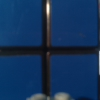
\includegraphics[scale=0.4]{calibrage0}
	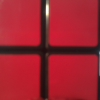
\includegraphics[scale=0.4]{calibrage1}
	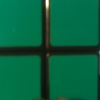
\includegraphics[scale=0.4]{calibrage2}
	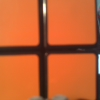
\includegraphics[scale=0.4]{calibrage3}
	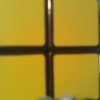
\includegraphics[scale=0.4]{calibrage4}
	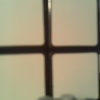
\includegraphics[scale=0.4]{calibrage5}
	\caption{les six photos d'un calibrage}
\end{figure}
    Calibrer le cube consiste à photographier les six faces du cube résolu pour connaitre l'angle de teinte moyen de chaque
couleur, la différence de luminosité entre le blanc et la couleur la plus claire et l'écart de luminosité entre les différents
endroits à photographier.
    On demande donc à l'utilisateur de photographier les six faces, et on prend une valeur moyenne pour chaque face,
que l'on transfère en hls.
\begin{lstlisting}
couleurs = []
for image in sorted(listdir()):
    liste = cc.image2couleur(image)
    moyenne = cc.rgb256_to_hls(cc.moyennepixels(liste))
    liste_hls = list(map(cc.rgb256_to_hls,liste))
    couleurs.append(moyenne)
\end{lstlisting}
Pour simplifier, on demande à l'utilisateur de photographier blanc en dernier.
On calcule ensuite la différence entre la luminosité de blanc et celle de la couleur la plus lumineuse.
\begin{lstlisting}
diffblanc = (couleurs[-1][1] + max(couleurs[:-1],key = lambda x:x[1])[1])/2
\end{lstlisting}

Le calibrage trie ensuite les couleurs par teinte (grâce à la fonction python sorted) en ajoutant à la fin la première valeur, la teinte en HLS étant circulaire
\begin{lstlisting}
couleurs = sorted([x[0] for x in couleurs[:-1]])
couleurs.append(couleurs[0]+1)
\end{lstlisting}
Dans la même boucle, on effectue une moyenne des écarts de luminosité entre les différents endroits étudiés

\begin{lstlisting}
exposition = [0,0,0,0]

for image in sorted(listdir()):
    liste = cc.image2couleur(image)
    liste_hls = list(map(cc.rgb256_to_hls,liste))
    exposition = [exp - pix[1] + moyenne[1]
                  for exp,pix in zip(exposition,liste_hls)]

exposition = [elem / 6 for elem in exposition]

\end{lstlisting}

Le calibrage nous renseigne aussi sur les couleurs opposées en stockant dans un dictionnaire pour chaque couleur en clé, son opposé en valeur.
Le blanc est défini par la chaine \texttt{"blanc"}
\begin{lstlisting}
def oppose(calibrage):
    dico = dict()
    for x in range(4):
        dico[calibrage[x][0]] = calibrage[(x+2)%4][0]
    dico["blanc"] = calibrage[4][0]
    dico[calibrage[4][0]] = "blanc"
    return dico
\end{lstlisting}

	\subsection{Sur la capture du cube}
	
\begin{figure}[h]
	\centering
	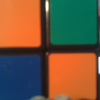
\includegraphics[scale=0.4]{cube0}
	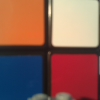
\includegraphics[scale=0.4]{cube1}
	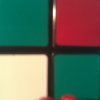
\includegraphics[scale=0.4]{cube2}
	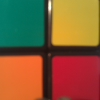
\includegraphics[scale=0.4]{cube3}
	\caption{les quatres photos nécessaires à la résolution du cube}
\end{figure}
    La capture se fait à partir de quatre photos car on peut déterminer, à partir de deux autocollants, quel sera le troisième, grâce à la parité. 
Cela permet de ne pas avoir à se questionner sur l'orientation à donner aux deux dernières photographies.
\begin{lstlisting}
def troisieme(coin,down):
    pattern = "DLBURF"
    position = [pattern.index(x)%3 for x in coin]
    horaire = not((position[0]-position[1])%3 - 1)
    parite = [x in pattern[3:] for x in coin]
    return pattern[3*((horaire + down + sum(parite))%2) + 3-sum(position)]
\end{lstlisting}

	On réalise la photographie du cube avec la base à plateau tournant, ce qui permet à la caméra de viser le centre des quatre autocollants présentés.
	\begin{figure}[h]
	\centering
	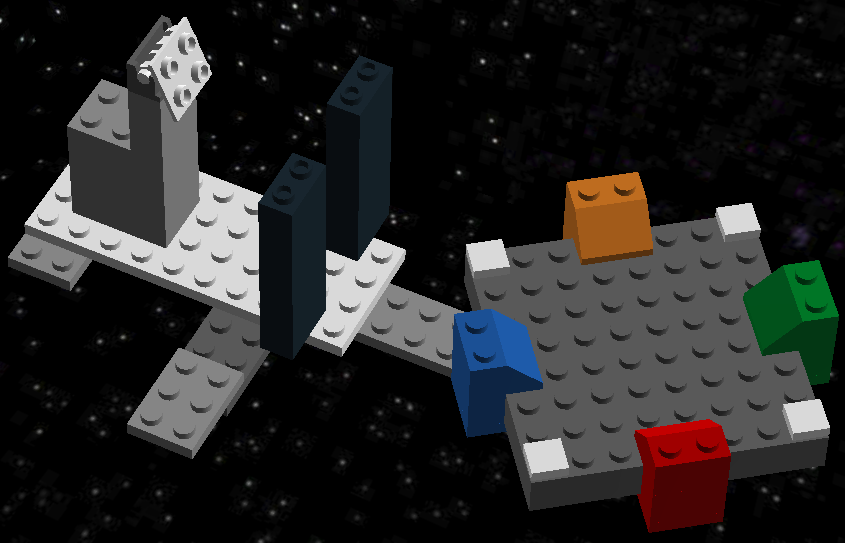
\includegraphics[scale=0.3]{support2x2x2raspi}
	\caption{la base à plateau tournant}
\end{figure}

	\subsection{De la couleur au cube}
    Pour passer de la couleur au cube, nous nous basons sur le coin au fond, en bas à gauche. Nous avons demandé
à l'utilisateur que l'autocollant en bas de ce coin soit le blanc. On utilise le dictionnaire des opposés pour
déterminer quelles couleurs vont devant, en haut et à droite.
\begin{lstlisting}
def tradstickerface(pieceDBL,oppose):
    dico = dict()
    for num,val in enumerate(["blanc"] + pieceDBL):
        dico[val] = "DBL"[num]
        dico[oppose[val]] = "UFR"[num]
    return dico
\end{lstlisting}
Nous extrayons tout d'abord un pixel de chaque autocollant photographié :
\begin{lstlisting}
def image2couleur(image):
    with Image.open(image) as photo:
        return [photo.getpixel((25+50*(x%2),25+50*(x>1))) for x in range(4)]
\end{lstlisting}
Pour chaque autocollant, on regarde si le pixel capturé est blanc :
Un pixel, après avoir ajouté l'écart à la moyenne, a une luminosité supérieure à la différence au blanc,
c'est que ce pixel provient d'un autocollant blanc.
Sinon, on cherche la couleur du calibrage la plus proche de celle capturée grâce à un algorithme récursif.
\begin{lstlisting}
def stickers(pixel,calibrage):
    if pixel[1] > calibrage[0]:
        return "blanc"
    else:
        v = plusproche(calibrage[1],pixel[0])
        return v - (v>1)

def plusproche(liste,valeur):
    milieu = floor(len(liste)/2)
    if milieu == 0:
        return liste[0]
    else:
        if (liste[milieu-1] + liste[milieu]) / 2 < valeur:
            return plusproche(liste[milieu:],valeur)
        else:
            return plusproche(liste[:milieu],valeur)
\end{lstlisting}
Par décalage et par déduction des faces du dessus et du dessous, on rassemble les autocollants par pièce.
\begin{lstlisting}
cube = [[face[:2] for face in cube],[face[2:] for face in cube]]
cube = [sum(semicube,[]) for semicube in cube]
traduction = cc.tradstickerface(cube[1][5:7],opposes)
cube = [[traduction[sticker] for sticker in moitie] for moitie in cube]
cube = cube[0][1:] + cube[0][0:1] + cube[1][1:] + cube[1][0:1]
liste = list()
for x in range(8):
    liste.append([cc.troisieme("".join(cube[2*x:2*x+2]),x>3)] +
                 cube[2*x:2*x+2])
cube = liste
cube[:4] = [stick[0:1]+stick[:0:-1] for stick in cube[:4]]
liste = liste[:2] + liste[3:1:-1] + liste[4:6] + liste[:5:-1]
\end{lstlisting}
Puis on construit un cube prêt à être utilisé par l'algorithme de résolution d'Alban
\begin{lstlisting}
import cube2 as mcube
cube = mcube.Cube()
for x in range(7):
    cube.set(mcube.corner(x),liste[x])

\end{lstlisting}


\section{Résoudre un cube}
 	\subsection{Un cube informatique}
    Nous avons eu besoin de trois classes pour résoudre le cube.
La classe \texttt{cube} est la classe décrivant un objet cube. Elle contient des chaînes de caractères nous renseignant
sur l'état du cube. Elle dispose de méthodes permettant d'effectuer des coups à un cube, d'obtenir l'inverse
d'un cube et de transformer un cube en nombre et un nombre en cube pour un stockage plus facile des données.
\par
La classe \texttt{sequence} décrit un objet contenant des coups à appliquer à un cube. Elle dispose d'une methode permettant
d'inverser une séquence (l'inverse de la séquence permettant de passer du cube A au cube B est celle permettant
de passer du cube B au cube A)
\par
La classe \texttt{collection} décrit enfin un objet contenant un ensemble de sequences.
	\subsection{Résolution}
Soit m le maximum de coups à rechercher.
La résolution se déroule en deux étapes. Tout d'abord, on cherche tous les cas possibles du cube résolu en
m/2 coups. Si parmi ces cubes, on trouve le cube à résoudre, on ressort l'inverse de la séquence ayant permis
de passer du cube résolu au cube à résoudre.
Sinon, on applique les séquences de 1 à n coups au cube à résoudre, et on regarde si le cube obtenu n'est
pas parmi les cubes obtenu en 6 coups à partir du cube résolu. Si c'est le cas, on ressort la première séquence
liée à l'inverse de celle utilisée pour obtenir le cube en 6 coups.
Sinon, c'est qu'il n'existe pas de solutions dont le nombre de coups soit inférieur à m pour résoudre le cube.


\section{Sur l'affichage 3D}

On compte encore une fois ici sur une bibliothèque de python appelée vpython (\emph{3D programming for simple mortals})
Nous utilisons deux objets : la boîte (box), on donne à cet objet trois coordonnées de position, trois coordonnées
de dimensions (hauteur,largeur,profondeur) et trois coordonnées de couleur (r,g,b).\\

On crée 8 boites (décoratives) représentant la structure du cube, de forme cubique,
\begin{lstlisting}
    for x in range(8):
        v.box(pos=(-.5+(x//2)%2,-.5+x//4,-.5+x%2),frame=cube[x],color=(.5,.5,.5))
\end{lstlisting}
et 24 boîtes très fines de couleurs différentes qu'on va venir poser sur la structure : les autocollants.
\begin{lstlisting}
    for x in range(4):
        v.box(pos=(-.5+x//2,-(1+stwth/2),-.5+x%2),
            length=stdim,height=stwth,width=stdim,
            frame=extraction["D"][x],color=v.color.white)
\end{lstlisting}
Pour lier trois autocollants à une pièce, on utilise l'objet frame, qui crée un objet contenant la structure
et les trois autocollants qui y sont collés. Les pièces ainsi crées sont stockées dans une liste selon leur position
\begin{lstlisting}
cube = [v.frame(display=image) for x in range(8)]
\end{lstlisting}

Pour faire tourner l'animation, on utilise la méthode rotate qui permet de faire tourner un objet autour
d'un vecteur donné d'un angle donné. On applique cette méthode à tous les objets se trouvant sur la face
à tourner avec un vecteur partant du centre de la face et pointant vers l'extérieur.
\begin{lstlisting}
def rotation_image(face,angle,anim = True):
    extractmaj()
    move=extraction[face]
    for x in range(int(FPS*SPEED)):
        for piece in move:
            piece.rotate(angle=(angle*v.pi/2)/(FPS*SPEED),
                         axis=axe[face])
\end{lstlisting}
Pour cela nous utilisons la fonction \texttt{extractmaj} qui extrait d'un côté les pièces d'une face donnée de la liste et de l'autre les pièces
de la face opposée,
\begin{lstlisting}
def extractmaj():
    global extraction
    extraction = {"D":cube[:4],
                  "L":cube[:2]+cube[4:6],
                  "B":cube[::2],
                  "U":cube[4:],
                  "R":cube[2:4]+cube[6:],
                  "F":cube[1::2]}
\end{lstlisting} 
et le dictionnaire \texttt{axe} qui associe à chaque face le vecteur allant du centre vers elle.
\begin{lstlisting}
axe = {"D":(0,-1,0),"L":(-1,0,0),
       "B":(0,0,-1),"U":(0,1,0),
       "R":(1,0,0), "F":(0,0,1)}
\end{lstlisting}
\par
Il faut ensuite faire tourner les pièces à l'intérieur de la liste, 
\begin{lstlisting}
    move,fixe = extraction[face],extraction[oppose[face]]
    move=move[:2]+move[:1:-1]
    if face in "ULF":
        move=tourne(move,-angle)
    else:
        move=tourne(move,angle)
\end{lstlisting}
Puis reconstruire le cube à l'aide des pièces de la face ayant tourné et des pièces de la face opposée restées fixes.
\begin{lstlisting}
    move=move[:2]+move[:1:-1] 
    reconstructeur = {"D":move+fixe,
                      "L":move[:2]+fixe[:2]+move[2:]+fixe[2:],
                      "B":move[0:1]+\
                      [(move[1:]+fixe)[x%7] for x in range(3,28,4)],
                      "U":fixe+move,
                      "R":fixe[:2]+move[:2]+fixe[2:]+move[2:],
                      "F":fixe[0:1]+\
                      [(fixe[1:]+move)[x%7] for x in range(3,28,4)]}
    cube = reconstructeur[face]
\end{lstlisting}

Pour l'animation, nous sommes partis du cube résolu, auquel nous avons appliqué la séquence inverse de la
séquence à résoudre, sans pause, d'où l'effet instantané, 
\begin{lstlisting}
    for face,nombre in sequence_inverse(sequence):
        rotation_image(face,wca_angles[nombre],anim = False)
        rotation_objet(face,wca_angles[nombre])
\end{lstlisting}
puis nous avons appliqué la séquence à résoudre au cube.
\begin{lstlisting}
    for face,nombre in sequence.split(","):
        rotation_image(face,wca_angles[nombre)]
        rotation_objet(face,wca_angles[nombre])
\end{lstlisting}

\begin{figure}[h]
	\centering
	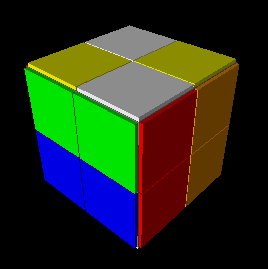
\includegraphics[scale=0.5]{capturevpython}
	\qquad
	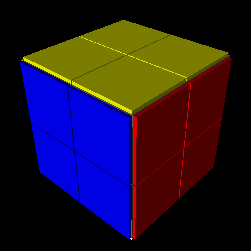
\includegraphics[scale=0.533]{captureresolu}
	\caption{le cube créé par vpython}
\end{figure}


\section*{Pour aller plus loin…}
Le futur proche de ce projet serait de faire correspondre la raspberry pi avec un ordinateur pour transmettre
le cube à résoudre ainsi que les couleurs du nano-ordinateur à l'ordinateur, pour gagner du temps, car la
raspberry pi ne dispose que de 512 Mio de RAM, ce qui est peu puissant, et aurait permis plus de liberté
dans la disposition du cube au moment de la capture.\\
Dans un lointain futur, nous aimerions pouvoir construire une machine capable de résoudre le cube elle-même
grâce à des moteurs, que l'on pourrait raccorder aux broches GPIO de la raspberry pi par exemple. Le lego
montre le début de ce projet.

\section*{remerciements}
Je tiens à remercier mes professeurs d'ISN M.Madec et Mme Durski, mon père qui a bien voulu investir dans une Raspberry pi, et Alban, qui a su me supporter lors du travail en groupe.

\end{document}